\documentclass[12pt, a4paper]{report}

\usepackage[utf8]{inputenc}
\usepackage{graphicx}
\usepackage{float}
\usepackage{listings}

\graphicspath{{../diagrams/images/}{../diagrams/images/png/}}

\title{Progetto Ingegneria del Software}
\author{Davide Bleggi \and Joshua Chapman}
\date{Giugno 2020}


\begin{document}
\begin{titlepage}
  \maketitle
\end{titlepage}

% Table of content
\tableofcontents
\newpage


\chapter{Introduzione}

Progetto per la creazione di un sistema informatico per gestire il servizio di
spesa online di un supermercato.

\section{Organizzazione}
% Subsection divisione del lavoro, tentativo di scrum, e difficoltà della 
% distanza
% Paired developement
Date le distanze, i tempi ristretti, e il nostro team composto da sole due
persone abbiamo preferito usare al \textbf{XP programming}, in grado di
adattarsi meglio alle nostre esigenze, e appoggiandoci ad un servizio di
\textbf{Version Control System} quale \textbf{GIT} per poter proseguire anche
in autonomia e non solo con l'ausilio del \textbf{pair programming}. Quindi
durante la progettazione è stato tenuto un approccio \textbf{Test First
Development} seguito da costanti aggiornamenti di \textbf{refactoring}.

\subsection{Analisi Dei Requisiti}
% Cominciato con analisi dei requisiti, sezioni del pdf
% Backlog dei requisiti
Prima di tutto abbiamo cominciato con l'analisi dei requisiti forniti dalla
documentazione. Quindi abbiamo estrapolato 6 macro sezioni principali:

\begin{itemize}
  \item Registrazione
    \begin{itemize}
      \item Gli utenti devono essere registrati.
      \item Ogni utente registrato accede con email e password.
      \item Gli utenti possono specificare un metodo di pagamento preferito.
    \end{itemize}
  \item Catalogo
    \begin{itemize}
      \item Se un utente inserisce un prodotto che al momento della conferma
        della spesa non risulta più disponibile,il sistema segnala la cosa al
        cliente ed elimina il prodotto dal carrello.
      \item Ogni utente registrato accede con email e password.
      \item Gli utenti possono specificare un metodo di pagamento preferito.
      \item Dopo aver confermato la spesa, l’utente sceglie data e orario della
        consegna visualizzando le opzioni possibili.
    \end{itemize}
  \item Carrello
    \begin{itemize}
      \item L’utente può visualizzare il carrello per modificare la quantità
        dei prodotti inseriti o rimuovere qualche prodotto.
      \item L’utente può ricercare i prodotti per tipo (uova, biscotti, pasta),
        per marca o per eventuali caratteristiche.
    \end{itemize}
  \item Effettua spesa
    \begin{itemize}
      \item Ad ogni spesa vengono accreditati sulla tessera fedeltà un numero
        di punti pari agli euro spesi nella spesa considerata.
    \end{itemize}
  \item Profilo utente
    \begin{itemize}
      \item Il sistema deve permettere agli utenti di accedere al loro profilo,
        modificare i dati anagrafici, verificare il saldo punti e lo stato
        delle loro spese.
      \item Ogni utente può vedere tutte le spese che ha effettuato nel tempo
        con il dettaglio dei prodotti acquistati.
    \end{itemize}
  \item Responsabili reparto
    \begin{itemize}
      \item Il sistema deve permettere agli utenti di accedere al
        loro profilo, modificare i dati anagrafici, verificare il saldo
        punti e lo stato delle loro spese.
      \item Ogni utente può vedere tutte le spese che ha effettuato nel tempo
        con il dettaglio dei prodotti acquistati.
      \item I responsabili del reparto spesa online devono autenticarsi per
        poter accedere al sistema e devono poter verificare lo stato delle
        spese e provvedere all’inserimento delle informazioni relative ai
        prodotti.
    \end{itemize}
\end{itemize}

% Subsection framework e librerie usati spring per il server e okhttp3. Javafx
% build system gradle
\subsection{Framework}

Per il progetto si sono ritenuti necessarie una serie di implementazioni di
librerie esterne.

\subsubsection{Spring}

Abbiamo utilizzato Spring (by Netflix) per un rapido sviluppo di un server
compatibile con Java.

\subsubsection{Okhttp3}

Per la comunicazione tra client e Server, abbiamo optato per un libreria in 
grado di gestire le richieste http per creare una web application.

\subsubsection{JavaSQL}

Per la gestione del database javaSQL con il driver di SQLite.

\subsubsection{JavaFX}

Per l'interfaccia grafica è stato utilizzato JavaFX.\@ Scelta perché è il più 
moderno e permette di essere utilizzato senza ausilio di librerie esterne.

\subsubsection{Gradle}
Utilizzato per la Build System modulare e per facilitare la compilazione
crossplatform (importando automaticamente le librerie necessarie).

\chapter{Design del Progetto}

\section{Use Cases}

\begin{figure}[h]
  \centering
  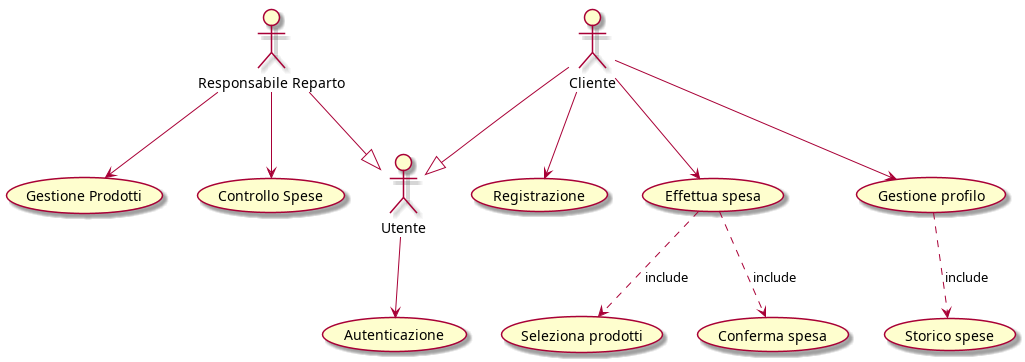
\includegraphics[width=\textwidth]{use_case_diagram.png}
  \caption{Use case diagram}
\end{figure}

Nel sistema abbiamo identificato 8 use cases. Gli attori necessari per il 
sistema sono i seguenti:

\begin{itemize}
  \item Clienti
  \item Responsabili Reparto
  \item Utente
\end{itemize}

I due attori Cliente e Responsabile Reparto sono generalizzati nel attore
Utente per tutti gli use case di autenticazione, in quanto andranno ad
autenticarsi nello stesso portale. Gli use case possono essere raggruppati in
base all'attore a cui appartengono. Le funzioni principali del responsabile
reparto sono di gestire prodotti e lo stato delle spese; gli use case del
cliente sono di registrarsi alla piattaforma, effettuare spese e gestire il
proprio profilo. Per tutti gli use case diversi dalla autenticazione o
registrazione, prendiamo come presupposto che l'utente sia già autenticato.

\subsection{User Use Cases}

Le seguenti sono gli use case del utente con i corrispettivi sequence diagrams.

\subsubsection{Autenticazione}

\begin{figure}[h]
  \centering
  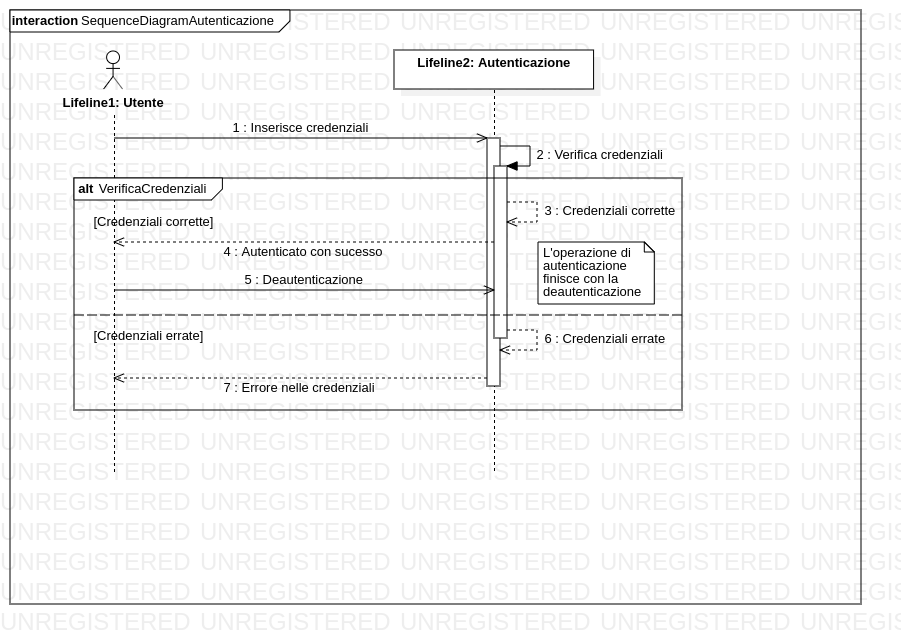
\includegraphics[width=\textwidth]{Use Case Model!Autenticazione!InteractionAutenticazione!SequenceDiagramAutenticazione_7.png}
  \caption{Sequence diagram autenticazione}
\end{figure}

Quando l'utente deve autenticarsi, inserisce le credenziali nel portale. Queste
verranno verificate. Nel caso siano corrette verrà autenticato con successo, e
potrà successivamente compiere il logout. Nel caso siano incorrette verrà
restituito un errore.

\newpage

\subsection{Responsabile Use Cases}

Le seguenti sono gli use case del responsabile del reparto con i corrispettivi 
sequence diagrams.

\subsubsection{Gestione Prodotti}

\begin{figure}[h]
  \centering
  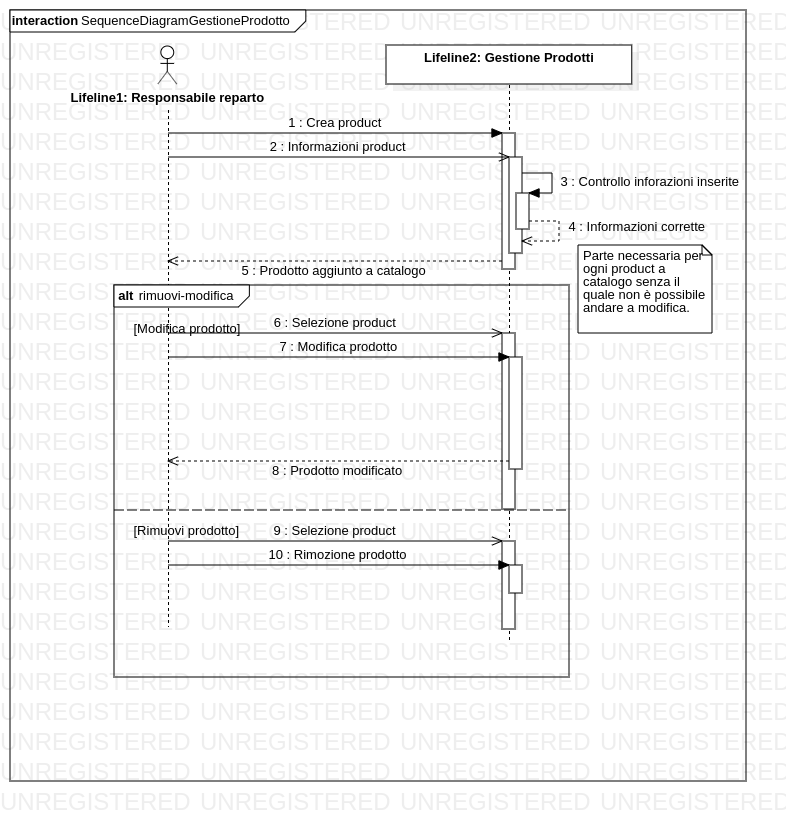
\includegraphics[width=\textwidth]{Use Case Model!Gestione prodotti!InteractionGestioneProdotti!SequenceDiagramGestioneProdotto_9.png}
  \caption{Sequence diagram gestione prodotti}
\end{figure}

Per la gestione dei prodotti il responsabile ha la possibilità di creare un
nuovo prodotto, modificarne o rimuoverne uno già esistente. La vista iniziale è
una lista dei prodotto, il responsabile può selezionarne uno e decidere se
modificarlo o rimuoverlo direttamente.

\subsubsection{Controllo Spese}

\begin{figure}[h]
  \centering
  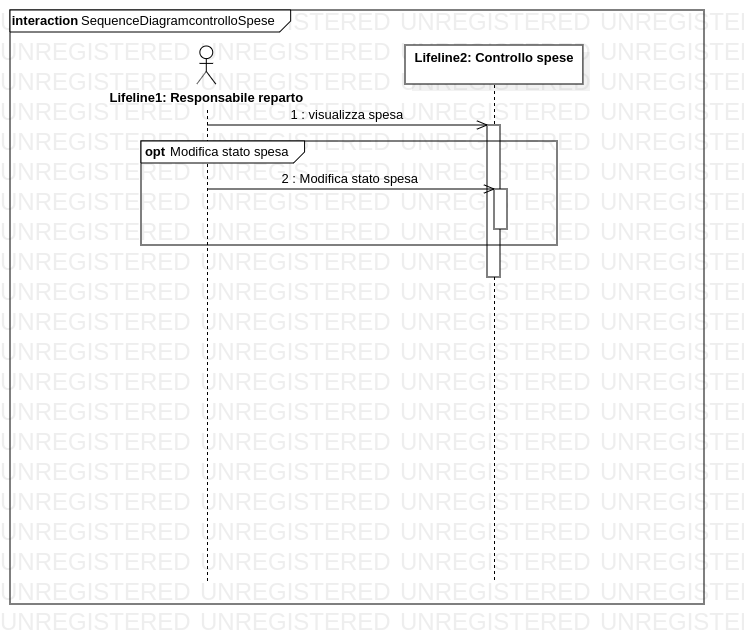
\includegraphics[width=\textwidth]{Use Case Model!Controllo spese!InteractionConstrolloSpese!SequenceDiagramcontrolloSpese_11.png}
  \caption{Sequence diagram controllo spese}
\end{figure}

In fine per il controllo delle spese il responsabile ne visualizza una lista
con tutte le informazioni riguardanti ogni ordine e ha la possibilità di
modificare lo stato delle spese nella lista.

\newpage

\subsection{Client Use Cases}

Le seguenti sono gli use case del cliente con i corrispettivi sequence diagrams.

\subsubsection{Registrazione}

\begin{figure}[h]
  \centering
  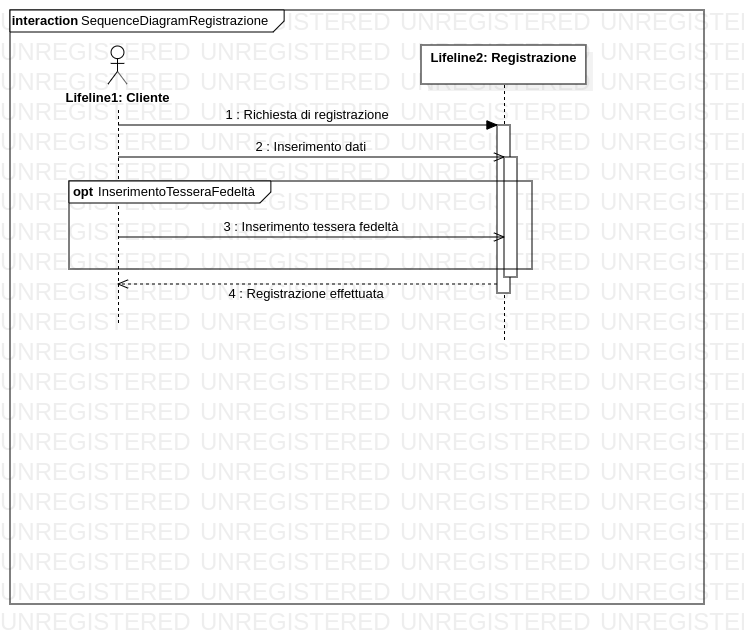
\includegraphics[width=\textwidth]{Use Case Model!Registrazione!InteractionRegistrazione!SequenceDiagramRegistrazione_1.png}
  \caption{Sequence diagram registrazione}
\end{figure}

Il cliente accede alla vista della registrazione e dopo aver inserito i propri
dati ha la possibilità di inserire una tessera di fedeltà, facoltativa.

\newpage

\subsubsection{Effettua Spesa}

\begin{figure}[h]
  \centering
  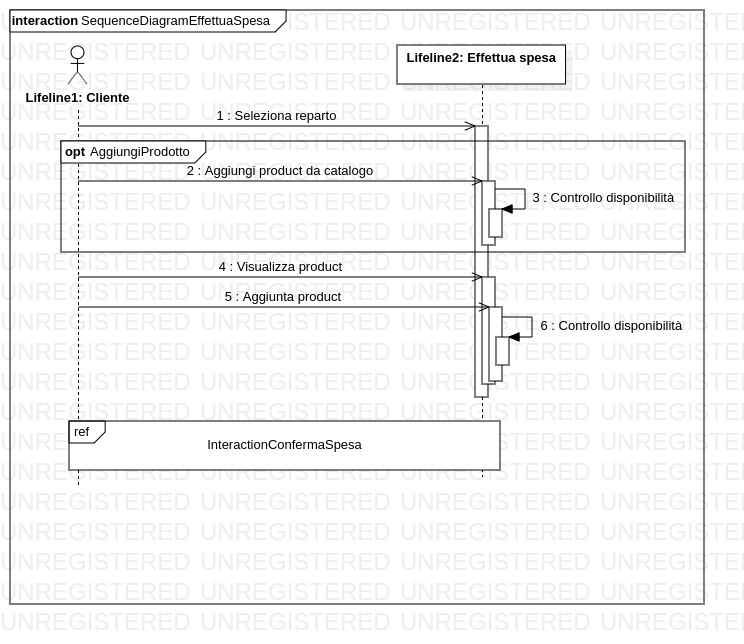
\includegraphics[width=\textwidth]{Use Case Model!Effettua spesa!InteractionEffettuaSpesa!SequenceDiagramEffettuaSpesa_3.png}
  \caption{Sequence diagram effettua spesa}
\end{figure}

Per effettuare la spesa il cliente prima visualizza il catalogo dei prodotti.
Qui può selezionare le diverse categorie o cercare i prodotti che vuole
aggiungere al carrello.

\newpage

\subsubsection{Conferma Spesa}

\begin{figure}[h]
  \centering
  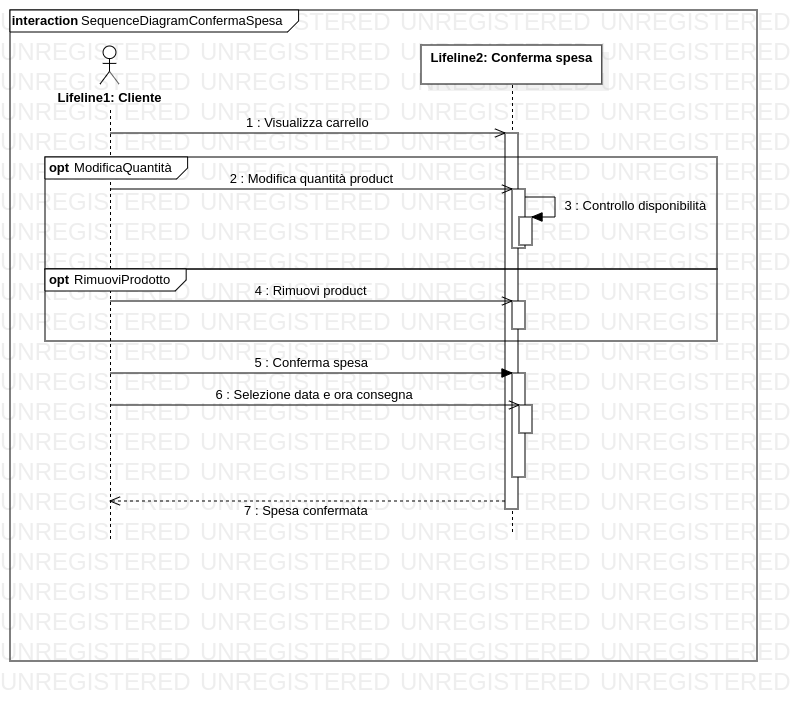
\includegraphics[width=\textwidth]{Use Case Model!Conferma spesa!InteractionConfermaSpesa!SequenceDiagramConfermaSpesa_13.png}
  \caption{Sequence diagram conferma spesa}
\end{figure}

Quando ha aggiunto almeno un prodotto al carrello può visualizzarli e
modificarne la quantità o rimuoverli. Quando ha tutti i prodotto che gli
servono può confermare l'ordine e selezionare una data e un ora per la
consegna.

\newpage

\subsubsection{Gestione Profilo}

\begin{figure}[h]
  \centering
  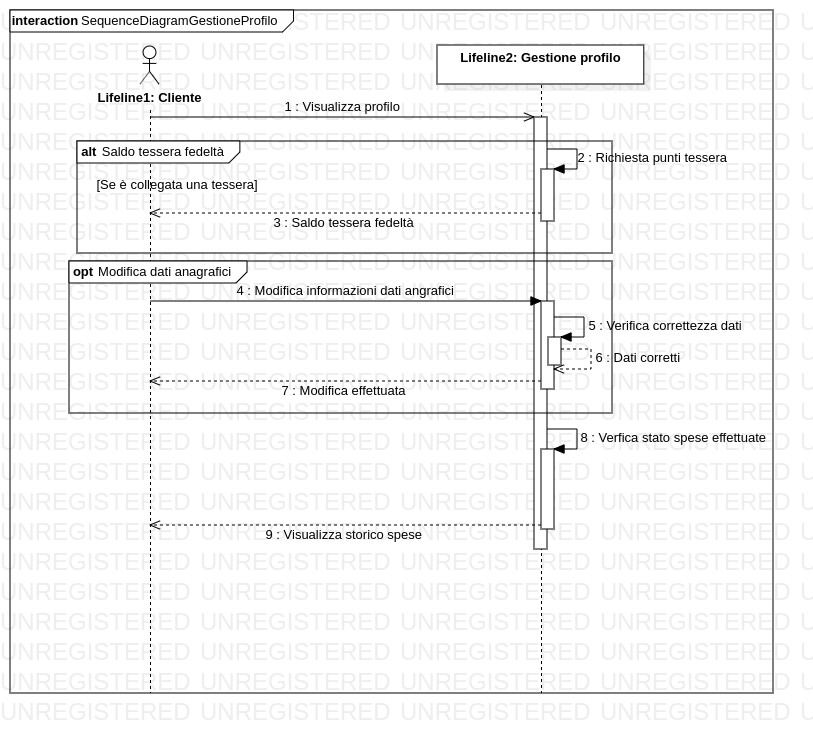
\includegraphics[width=\textwidth]{Use Case Model!Gestione profilo!InteractionGestioneProfilo!SequenceDiagramGestioneProfilo_5.png}
  \caption{Sequence diagram gestione profilo}
\end{figure}

Nella gestione del profilo il cliente può vedere le proprie informazioni
anagrafiche e modificarle. Inoltre se ha registrato una tessera fedeltà, sarà
possibile vedere il saldo dei punti guadagnati. Dalla visualizzazione del
profilo sarà possibile anche navigare alla visualizzazione dello storico delle
spese.

\newpage

\section{Activity diagram}

Di seguito sono riportati gli activity diagram delle principali funzioni che
dovrà avere il sistema.

% Activity diagram e spiegazione
\subsection{Autenticazione}

Il \textbf{cliente o il responsabile del reparto} inseriscono le credenziali
username e password. Il sistema le controlla e ritorna un messaggio di errore
se queste sono scorrette, altrimenti crea una sessione che si occuperà della
deautenticazione nel caso di Logout.\footnote{Nell'implementazione finale è
stato aggiunto un salvataggio della sessione, quindi con la chiusura
dell'applicazione non si raggiungerà necessariamente alla deautenticazione e
quindi alla conclusione del Activity Diagram}.

\begin{figure}[h]
  \centering
  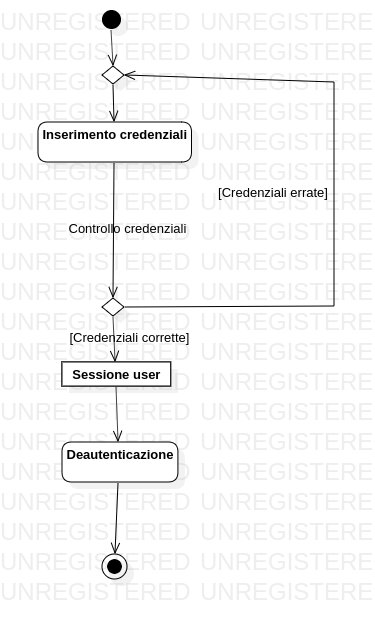
\includegraphics[width=0.52\textwidth]{Use Case Model!Autenticazione!ActivityAutenticazione!ActivityDiagramAutenticazione_8.png}
  \caption{Activity diagram autenticazione}
\end{figure}

\newpage

\subsection{Conferma Spesa}

Il \textbf{cliente} registrato un Visualizza il proprio carrello. Una volta
all'interno del carrello può Modificare le quantità, rimuovere il prodotto o
confermare la spesa. Se modifica le quantità bisogna tener in considerazione la
quantità di prodotti disponibili. Altrimenti se conferma bisognerà richiedere
le informazioni per la consegna.\footnote{Il metodo di pagamento viene
ottenuto direttamente dalla session dell'utente}

\begin{figure}[h]
  \centering
  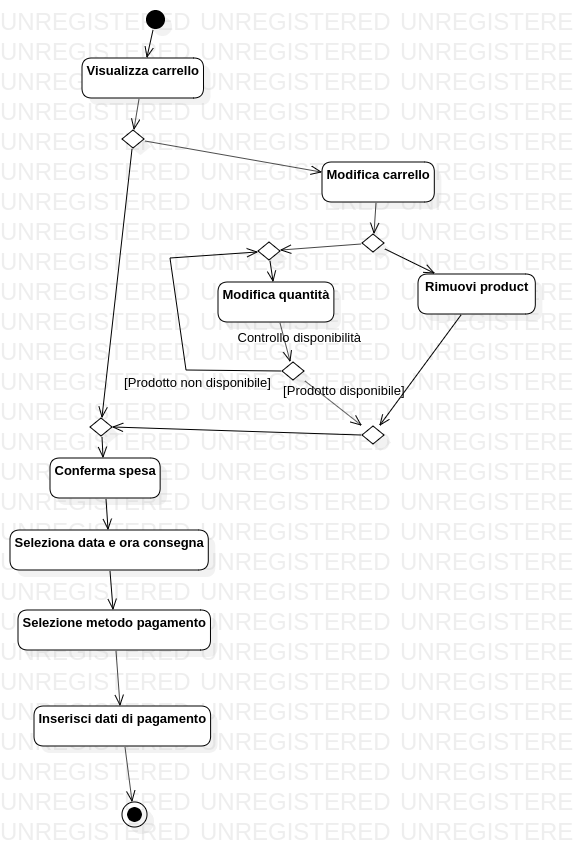
\includegraphics[width=0.73\textwidth]{Use Case Model!Conferma spesa!ActivityConfermSpesa!ActivityDiagramConfermaSpesa_14.png}
  \caption{Activity diagram Conferma Spesa}
\end{figure}

\newpage

\subsection{Visualizza Spesa}

Il \textbf{responsabile di reparto} una volta autenticato e all'interno della
visualizzazione della spesa, il responsabile può visualizzarne i prodotti di
una spesa o aggiornarne lo stato.

\begin{figure}[h]
  \centering
  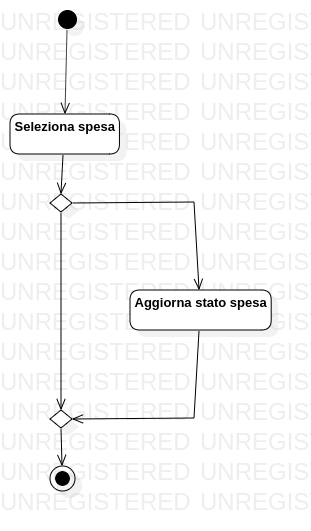
\includegraphics[width=0.64\textwidth]{Use Case Model!Controllo spese!ActivityControlloSpese!ActivityDiagramControlloSpese_12.png}
  \caption{Activity diagram Visualizza Spese}
\end{figure}

\newpage

\subsection{Effettua Spesa}

Il \textbf{cliente} una volta autenticato e all'interno del catalogo potrà
selezionare un reparto (di default preselezionato su All, contente tutti i
prodotti a catalogo) e potrà aggiungere prodotti al carrello sia dalla lista
del catalogo direttamente sia cliccando sul item corrispondente e
aggiungiendolo al carrello una volta aperta la scheda del prodotto
corrispondente. Prima dell'aggiunta il sistema controlla la disponibilità del
prodotto e se è disponibile lo aggiungie al carrello.

\begin{figure}[h]
  \centering
  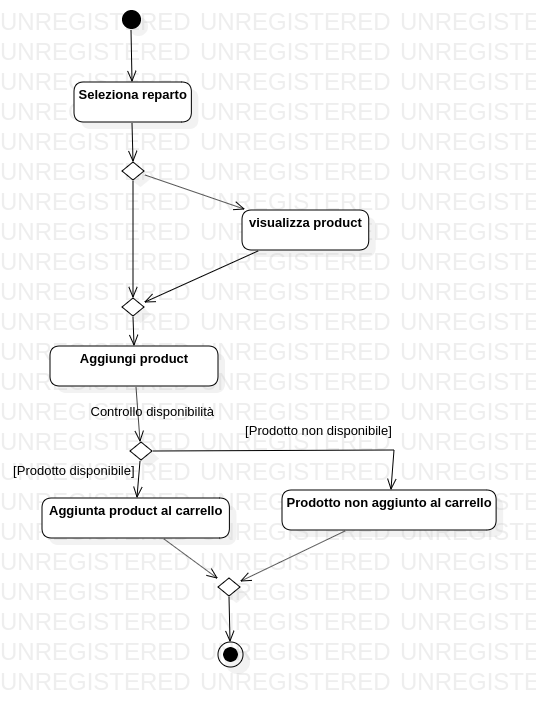
\includegraphics[width=0.8\textwidth]{Use Case Model!Effettua spesa!ActivityeffettuaSpesa!ActivityDiagramEffettuaSpesa_4.png}
  \caption{Activity diagram Effettua Spesa}
\end{figure}

\newpage

\subsection{Modifica/Aggiungi Prodotto}

Il \textbf{responsabile del reparto } una volta autenticato ed entrato nella
gestione dei prodotti potrà decidere se creare un nuovo prodotto o selezionarne
uno da catalogo per procedere alla modifica o alla rimozione. Nel caso di
creazione del prodotto inserisce le informazioni del prodotto che vengono
controllate dal sistema prima dell'aggiunta nel catalogo. Nel caso di modifica
della quantità o modifica del prodotto sarà possibile selezionare il prodotto
dalla lista. Una volta superati i controlli del sistema il prodotto verrà
aggiornato con le nuove informazioni.\footnote{Nell'implementazione è stata
aggiunta la opzione di selezionare il prodotto selezionandolo dalla lista}

\begin{figure}[h]
  \centering
  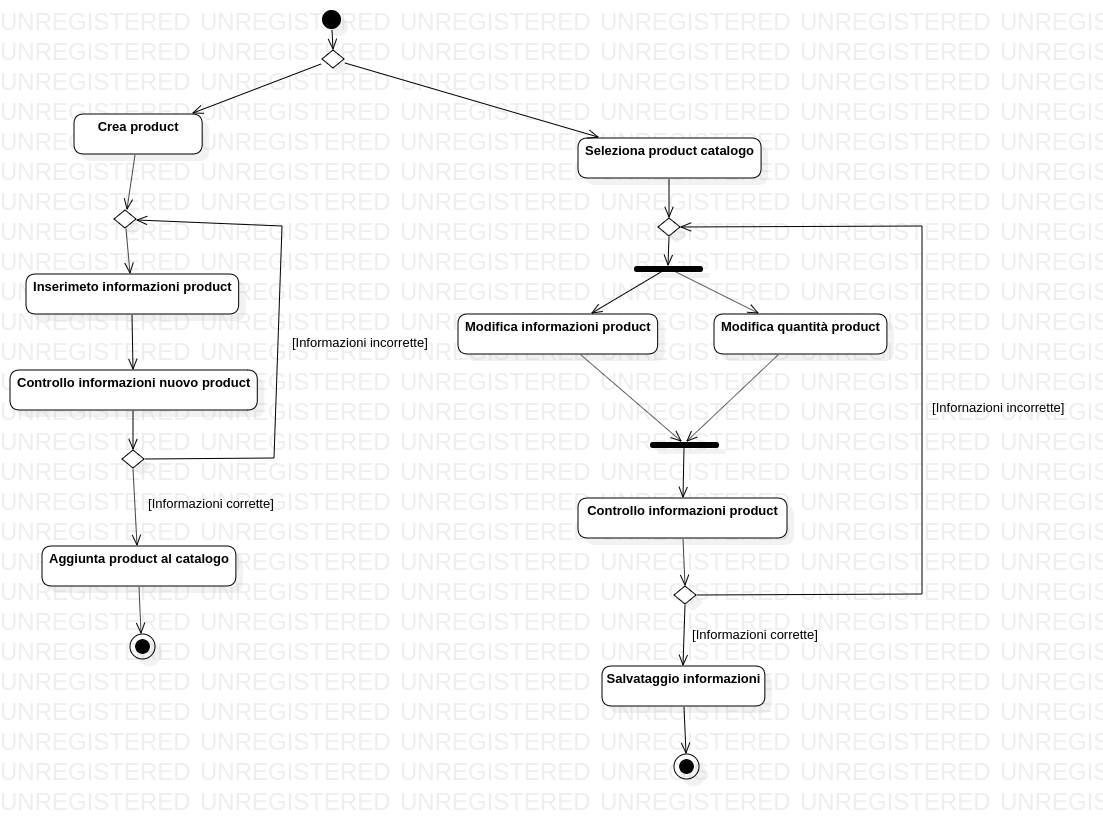
\includegraphics[width=\textwidth]{Use Case Model!Gestione prodotti!ActivityGestioneProdotti!ActivityDiagramGestioneProdotti_10.png}
  \caption{Activity diagram Modifica o Aggiungi Prodotto}
\end{figure}

\newpage

\subsection{Gestione Profilo}

Il \textbf{cliente} una volta autenticato e aver acceduto al proprio profilo
può modificare i propri dati o visualizzare lo stato delle proprie spese. Nel
caso di modifica dei dati il sistema provvederà alla verifica dei dati
inseriti. Se i dati risultano corretti allora i salva.

\begin{figure}[h]
  \centering
  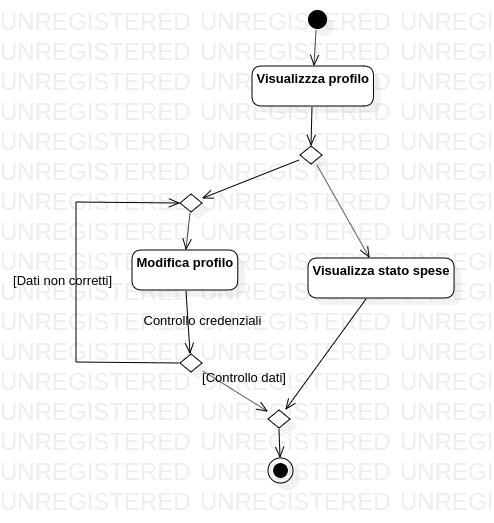
\includegraphics[width=\textwidth]{Use Case Model!Gestione profilo!Activity1!ActivityDiagramRegistrazione_6.png}
  \caption{Activity diagram Gestione Profilo}
\end{figure}

\newpage

\subsection{Registrazione}

Il \textbf{cliente} prima di autenticarsi entra in registrazione ed inserisce i
propri dati e se vuole la propria tessera fedeltà. Quindi il sistema verifica i
dati inseriti, se sono corretti registra il nuovo utente altrimenti segnala un
errore nella compilazione dei campi.

\begin{figure}[h]
  \centering
  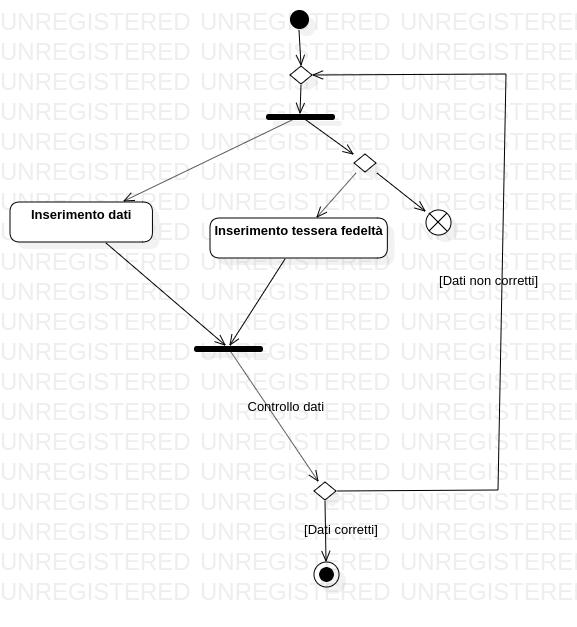
\includegraphics[width=\textwidth]{Use Case Model!Registrazione!ActivityRegistrazione!ActivityDiagramRegistrazione_2.png}
  \caption{Activity diagram Registrazione}
\end{figure}

\newpage

\section{Pattern Architetturali}

Il pattern architetturale principale del sistema è il Client e Server, mentre
sono stati utilizzati diversi pattern per i due rispettivi sistemi.

\subsection{MVC Model View Controller}

\begin{figure}[h]
  \centering
  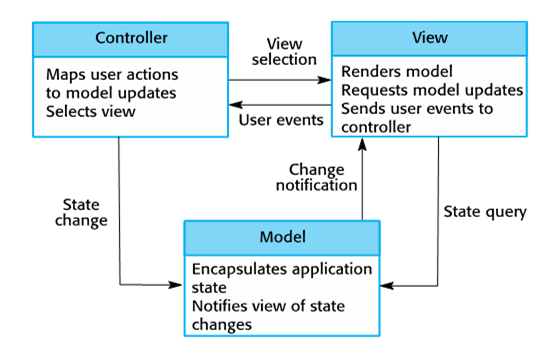
\includegraphics[width=\textwidth]{MVC.PNG}
  \caption{Schema Model View Controller}
\end{figure}

Il model View Controller è stato usato come pattern architetturale dato
dall'utilizzo implicito di questo sistema da parte di JavaFX.\@

\newpage

\subsection{Repository}

\begin{figure}[h]
  \centering
  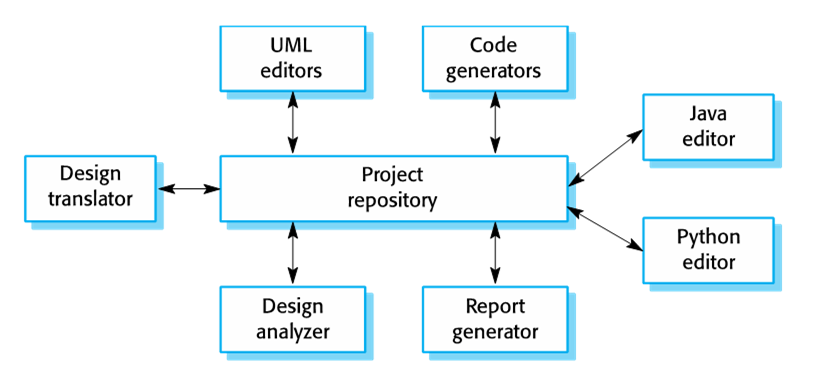
\includegraphics[width=\textwidth]{Repository.PNG}
  \caption{Schema esempio di una Repository}
\end{figure}

Il model Repository è stato utilizzato come pattern architetturale per la
gestione del database. 

\subsection{Client Server}

\begin{figure}[h]
  \centering
  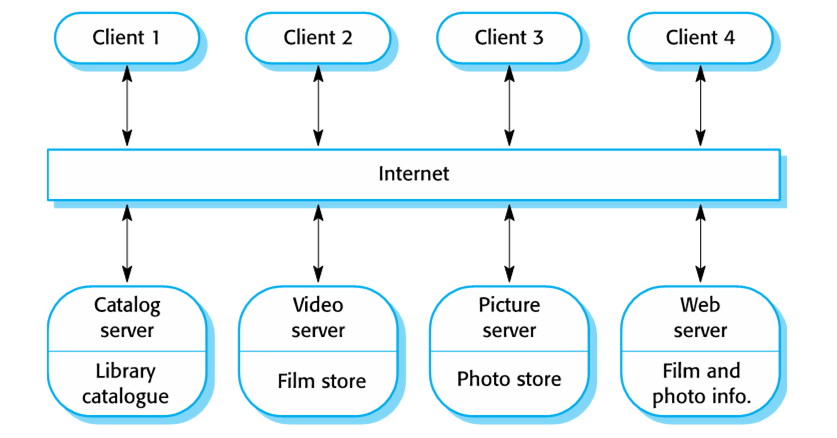
\includegraphics[width=0.8\textwidth]{Client-Server.PNG}
  \caption{Schema Client Server}
\end{figure}

Il Server Client è stato utilizzato come pattern architetturale di base per la
comunicazione col database.

\newpage

% MVC Server Repository(Database)

\section{Class diagram}

Le classi nel sistema rispecchiano il pattern architetturale. Possiamo
considerarle come due sistemi diversi del client e il server. 

Nel server ci sono due classi principali il Router, per la gestione delle
richieste e il Database, che controlla i modelli. Questi ultimi nel client sono
i model del MVC, mentre i controllers gestiscono l'esecuzione
dell'applicazione. Non tutti i campi dei model nel Database sono presenti anche
sul client, visto che sono utilizzati per facilitare il funzionamento del
database e non contengono vere informazioni.

Sia il server che il client contengono una classe Utils con solo metodi statici
che è stata crata per semplificare dei metodi e rende più modulare il codice.

\subsection{Server e Database}

\begin{figure}[h]
  \centering
  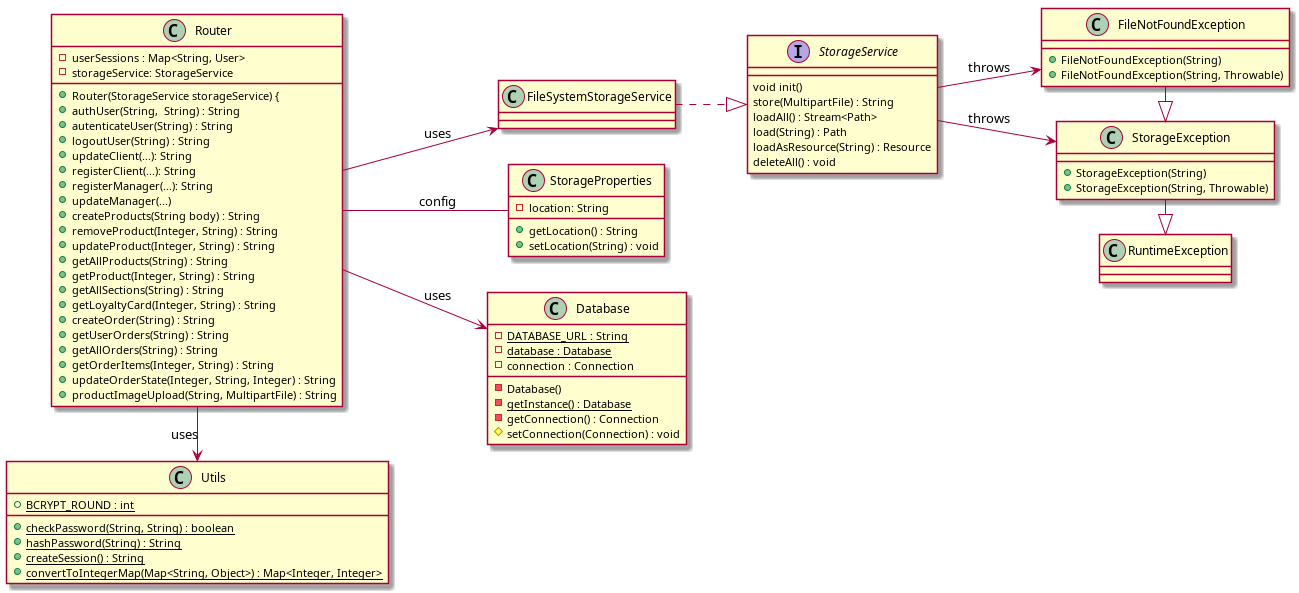
\includegraphics[width=\textwidth]{router_class.png}
  \caption{Class diagram server}
\end{figure}

Il Router ha il compito di gestire le chiamate del client e utilizza il
database e le classi dei model per ricavare le informazioni. In aggiunta al
database viene anche utilizzato lo FilesystemStorageService per salvare le
immagini dei prodotti caricate dagli utenti.

\newpage

\subsection{Models}

\subsubsection{Server}

Il database utilizza la classe Database per prendere una con\-nes\-sio\-ne al
da\-ta\-ba\-se fisico e i diversi models per ricavare le informazioni.

\begin{figure}[hb]
  \centering
  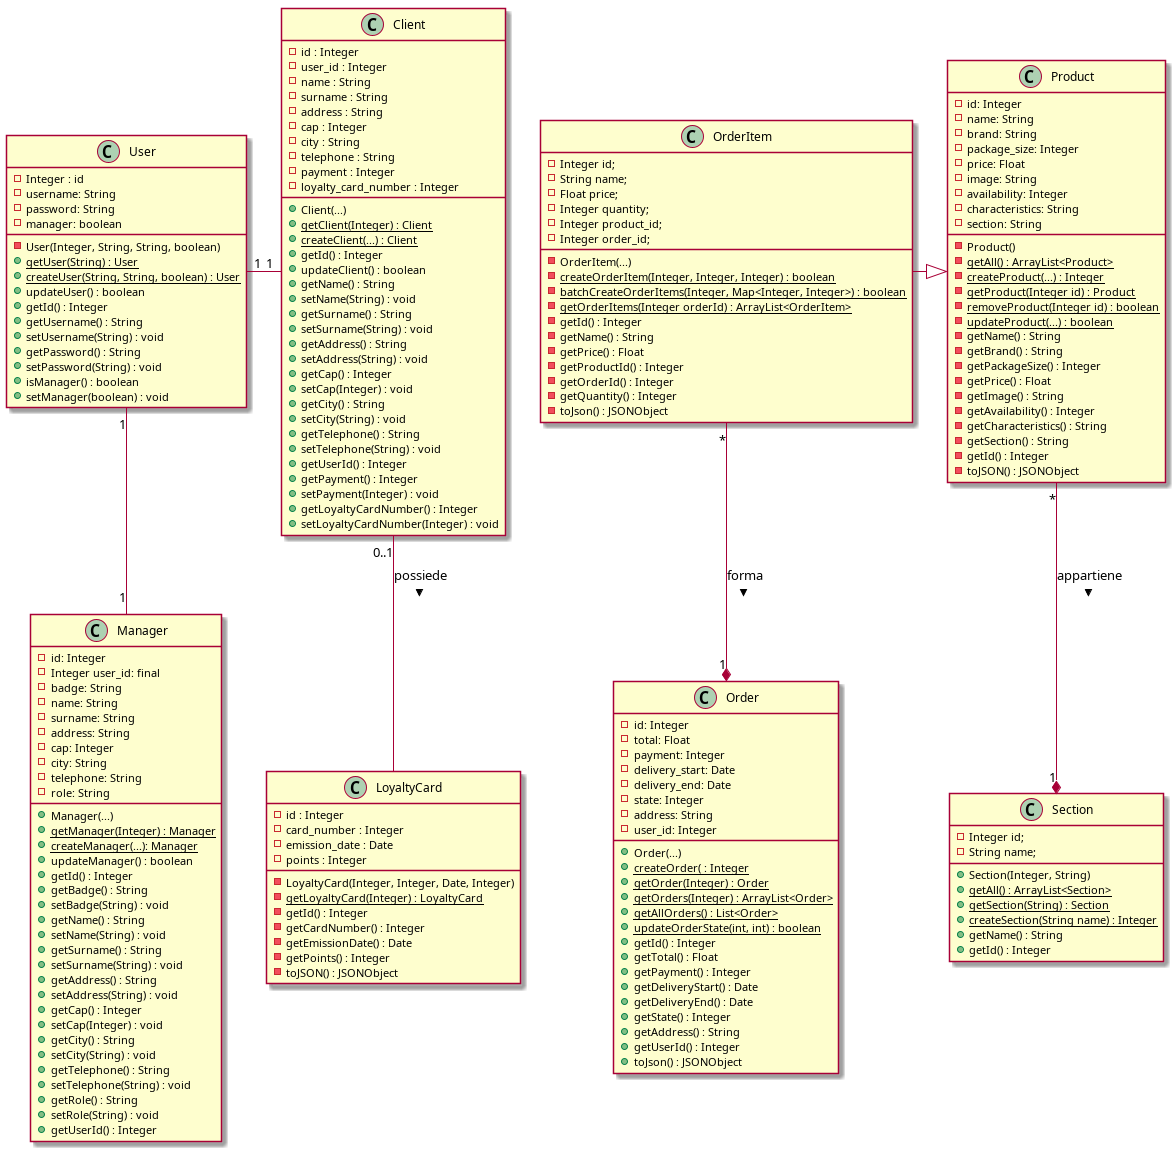
\includegraphics[width=\textwidth]{database_models_class.png}
  \caption{Class diagram database}
\end{figure}

\newpage

\subsubsection{Client}

Invece nel client la Section non è più necessaria e non dovendo più rispettare
lo schema del database possiamo creare una generalizzazione del User, Client e
Manager.

\begin{figure}[hb]
  \centering
  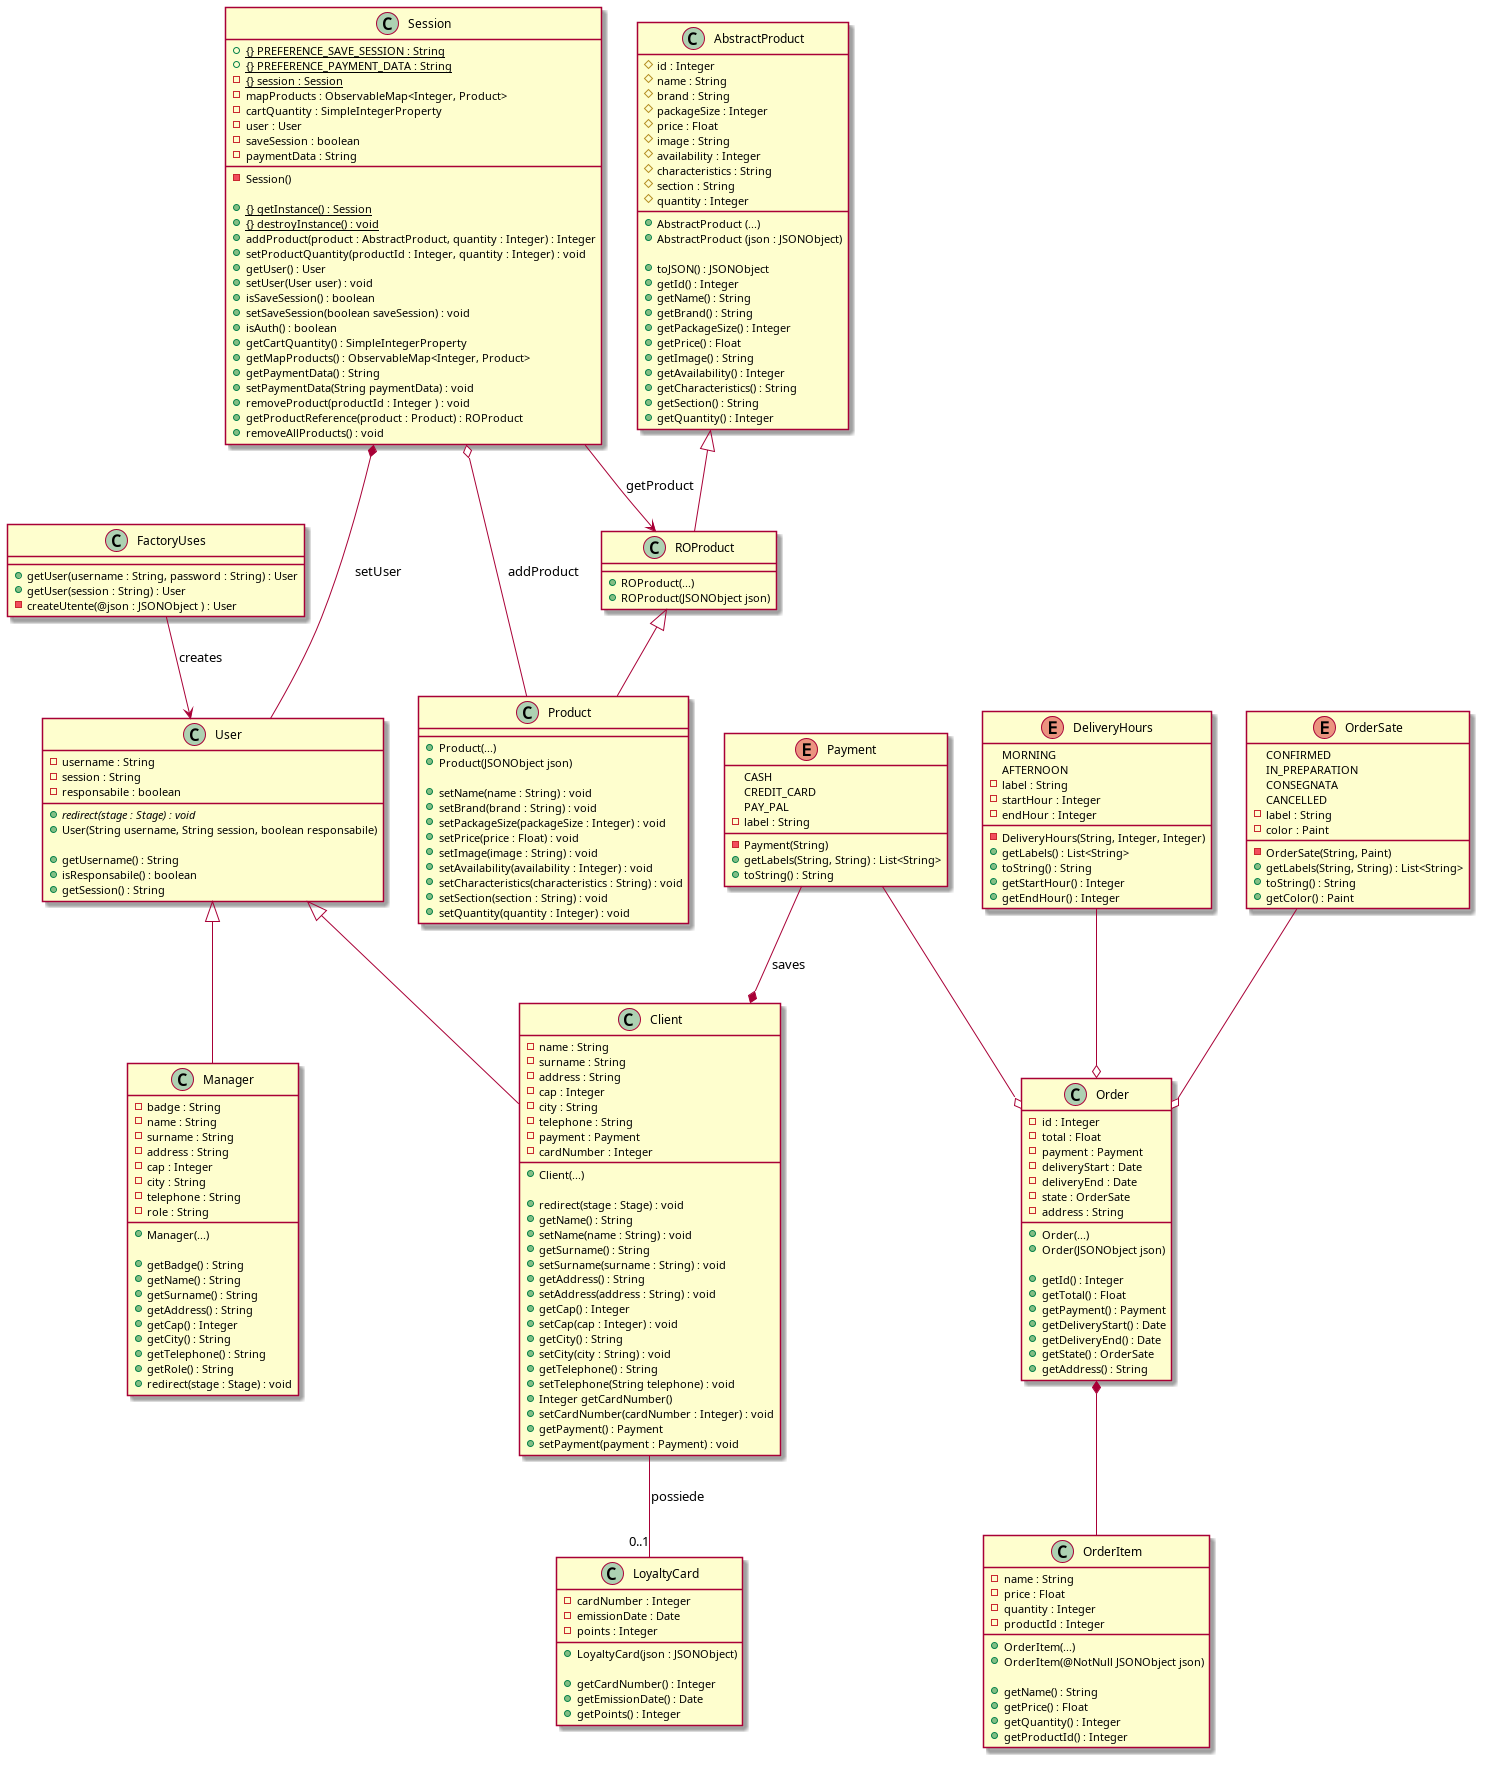
\includegraphics[width=0.9\textwidth]{client_models_class.png}
  \caption{Class diagram client}
\end{figure}

\newpage

% Classe della Sessione con eventuali robe

\subsection{Controllers}

\subsubsection{Autenticazione}

Per l'autenticazione l'utente inserisce le credenziali nel
AuthenticationController. Il controller passa le credenziali al FactoryUtente,
la cui funzione è di autenticare al server con le credenziali. Se ci sono
errori questi vengono riportati all'utente, altrimenti una sessione viene
ritornata dal server e utilizzata per creare l'istanza della classe User. La
sessione verrà mantenuta fino a quando l'utente non compie il log out.

\begin{figure}[h]
  \centering
  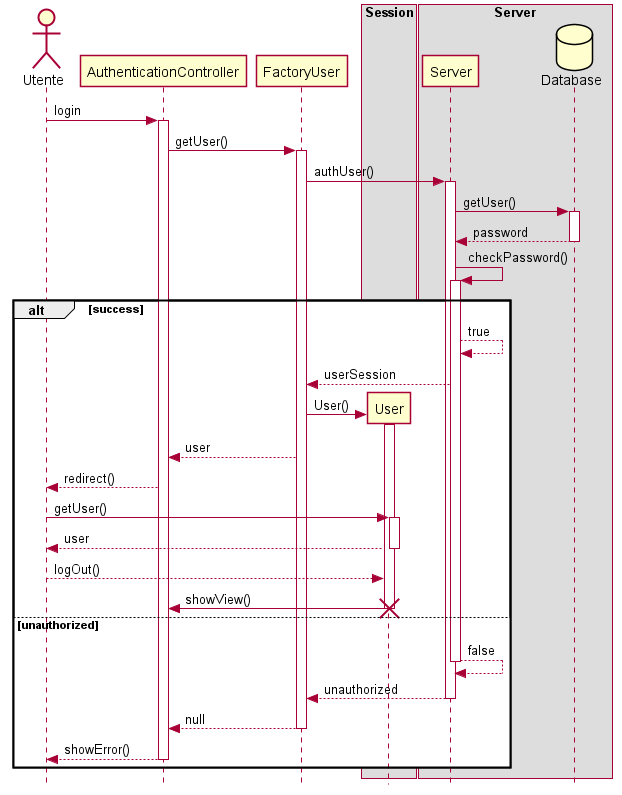
\includegraphics[width=0.8\textwidth]{auth_sequence.png}
  \caption{Sequence diagram Autenticazione}
\end{figure}

\newpage

\subsubsection{Gestione Profilo}

L'utente quando visualizza il proprio profilo utente ha l'opzione di modificare
i propri dati

\begin{figure}[h]
  \centering
  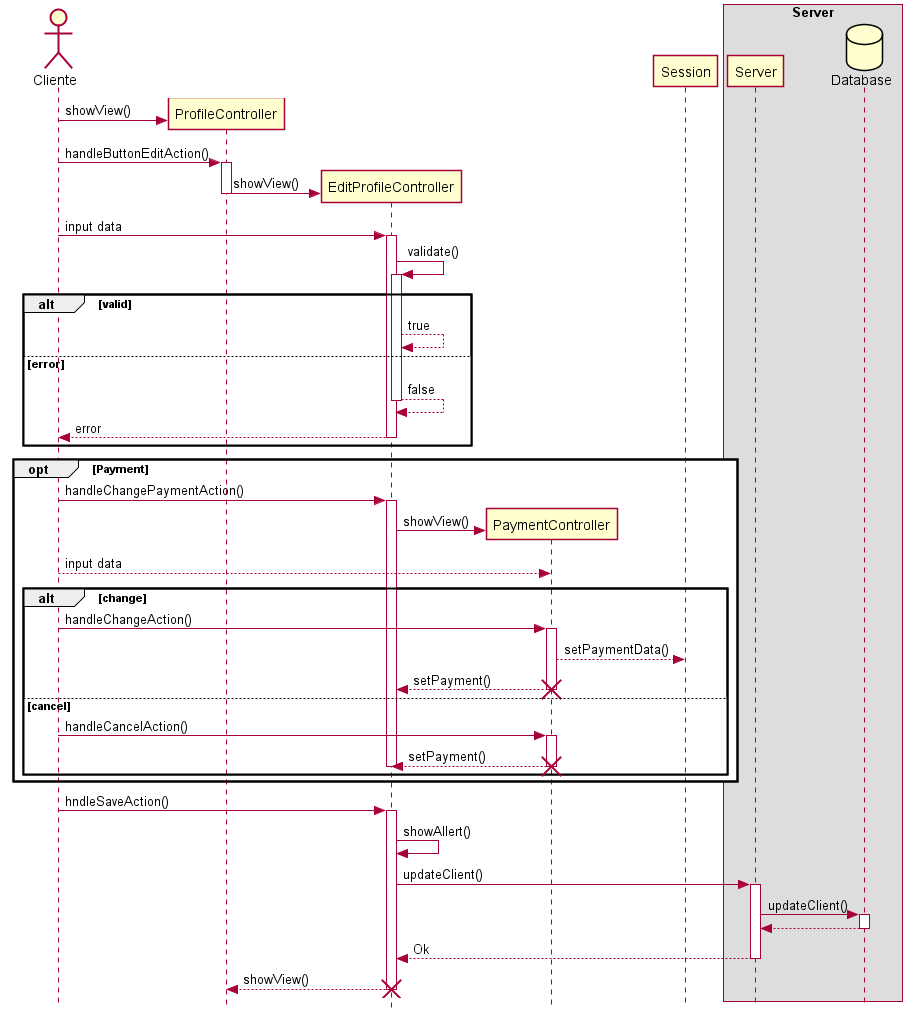
\includegraphics[width=0.9\textwidth]{profile_sequence.png}
  \caption{Sequence diagram Gestione Profilo}
\end{figure}

\newpage

\subsubsection{Registrazione}

\begin{figure}[ht]
  \centering
  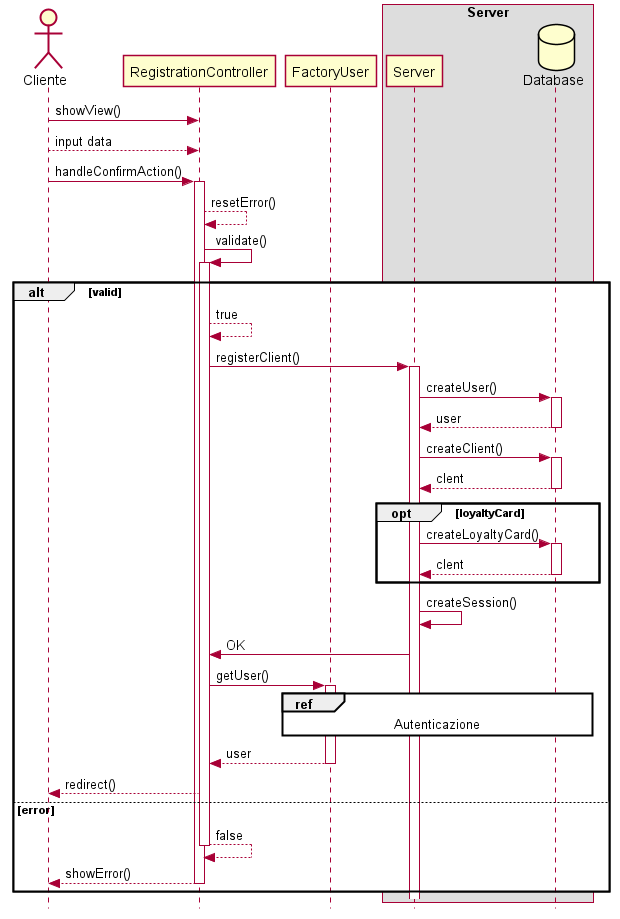
\includegraphics[width=0.7\textwidth]{registration_sequence.png}
  \caption{Sequence diagram Registrazione}
\end{figure}

\newpage

\subsubsection{Conferma Spesa}

\begin{figure}[ht]
  \centering
  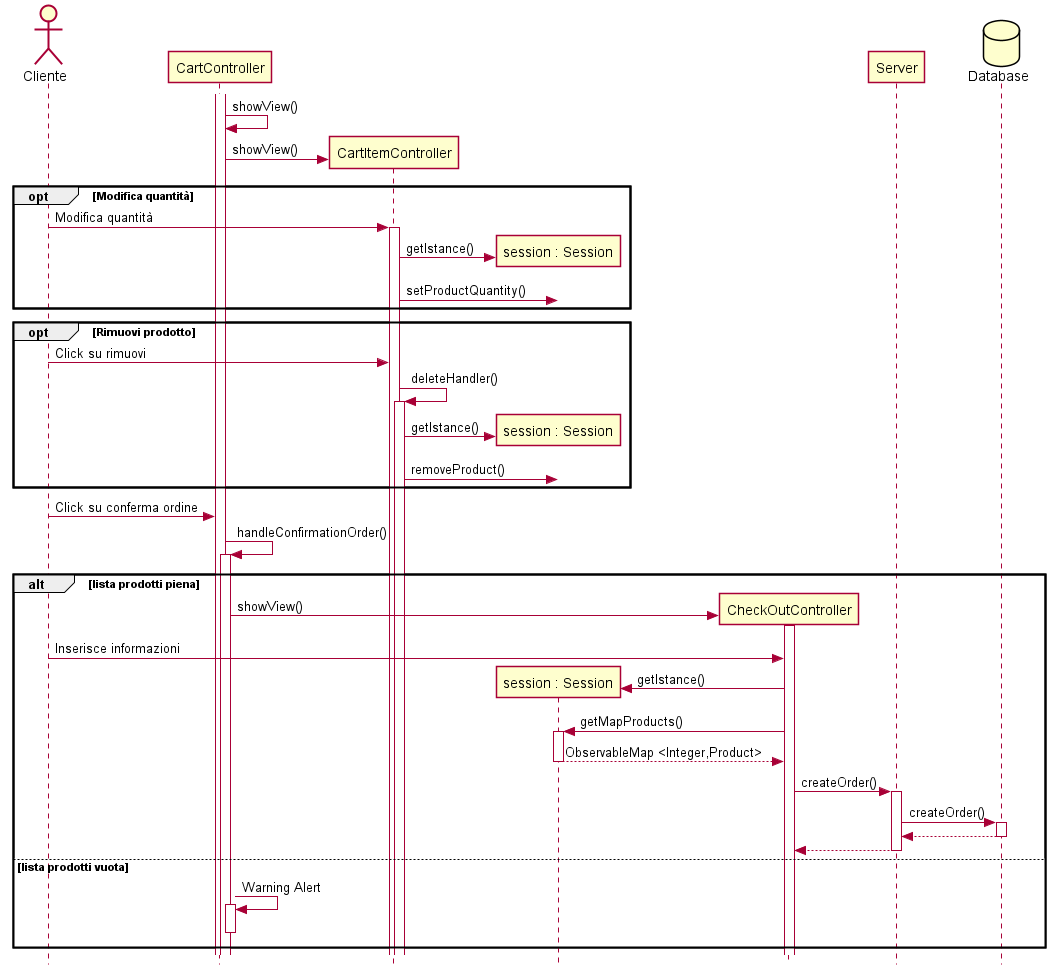
\includegraphics[width=0.9\textwidth]{sequence_conferma_spesa.png}
  \caption{Sequence diagram Conferma Spesa}
\end{figure}

\newpage

\subsubsection{Controlla Spese}

\begin{figure}[ht]
  \centering
  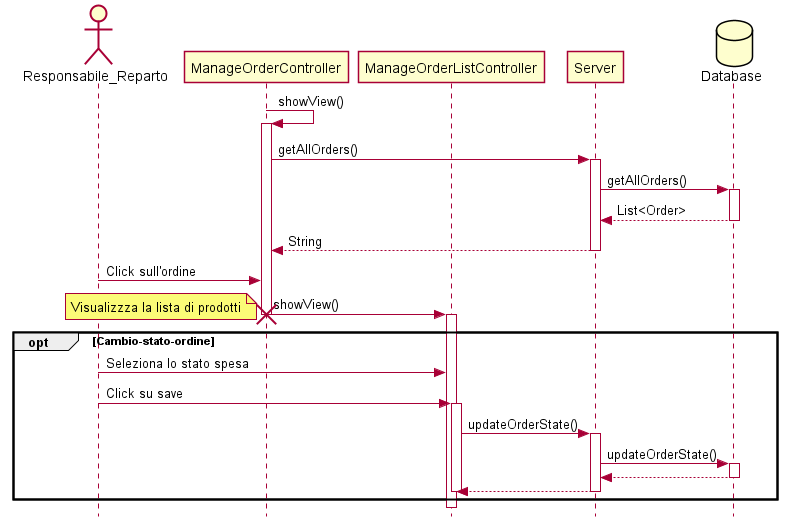
\includegraphics[width=0.9\textwidth]{sequence_controllo_spese.png}
  \caption{Sequence diagram Controlla Spese}
\end{figure}

\newpage

\subsubsection{Effettua Spesa}

\begin{figure}[ht]
  \centering
  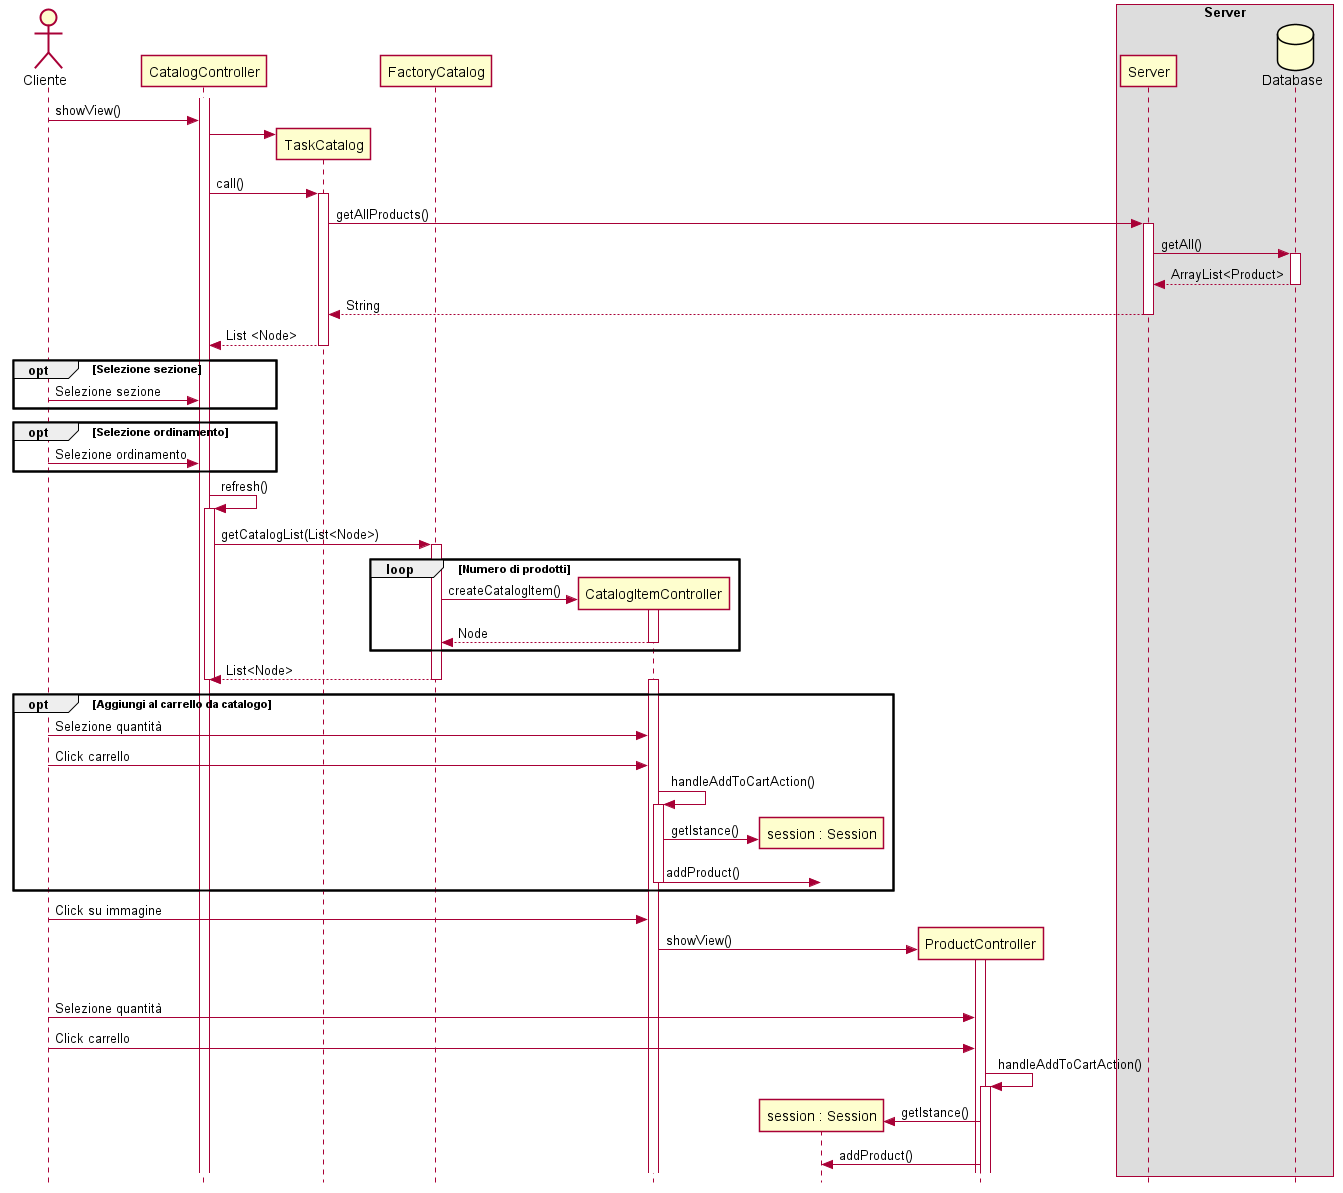
\includegraphics[width=0.9\textwidth]{sequence_effettua_spesa.png}
  \caption{Sequence diagram Effettua Spesa}
\end{figure}

\newpage

\subsubsection{Gestione Prodotti}

\begin{figure}[ht]
  \centering
  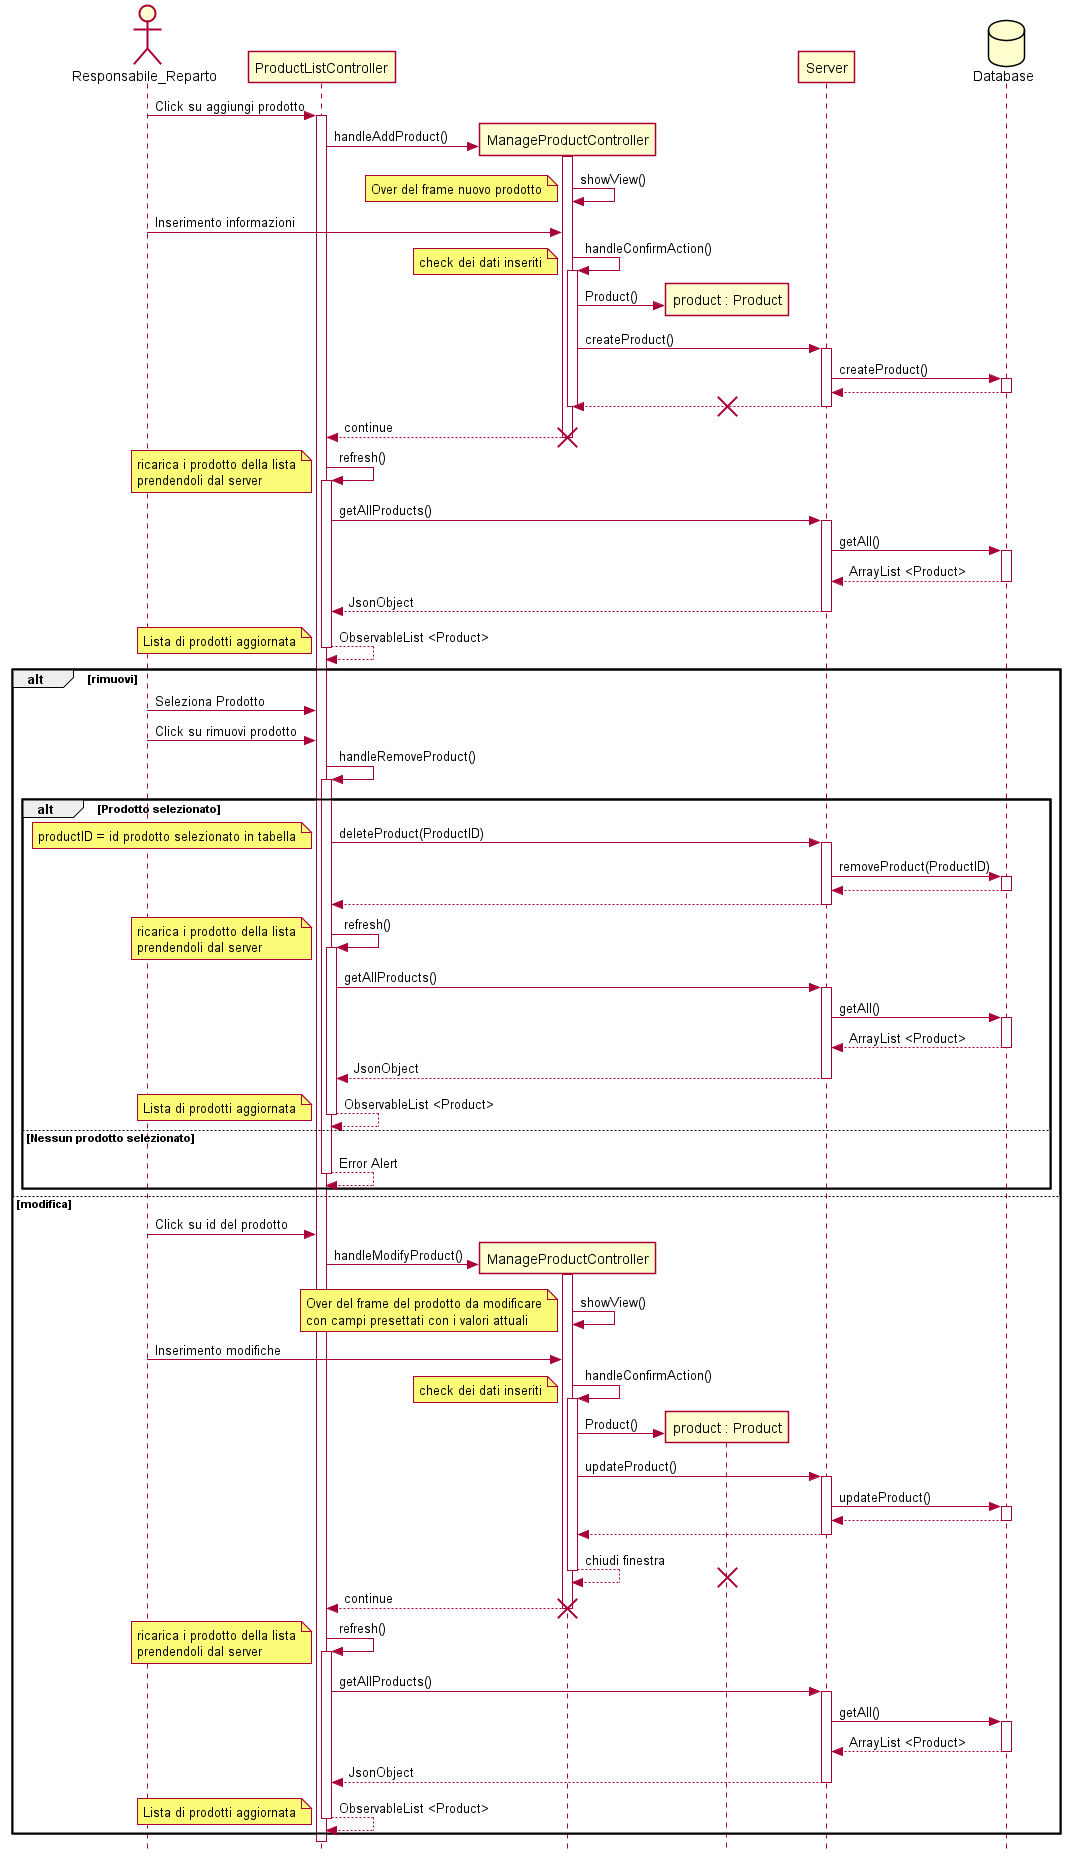
\includegraphics[width=0.6\textwidth]{sequence_gestione_prodotto.png}
  \caption{Sequence diagram Gestione Prodotti}
\end{figure}

\newpage

\subsubsection{Storico Spese}

\begin{figure}[ht]
  \centering
  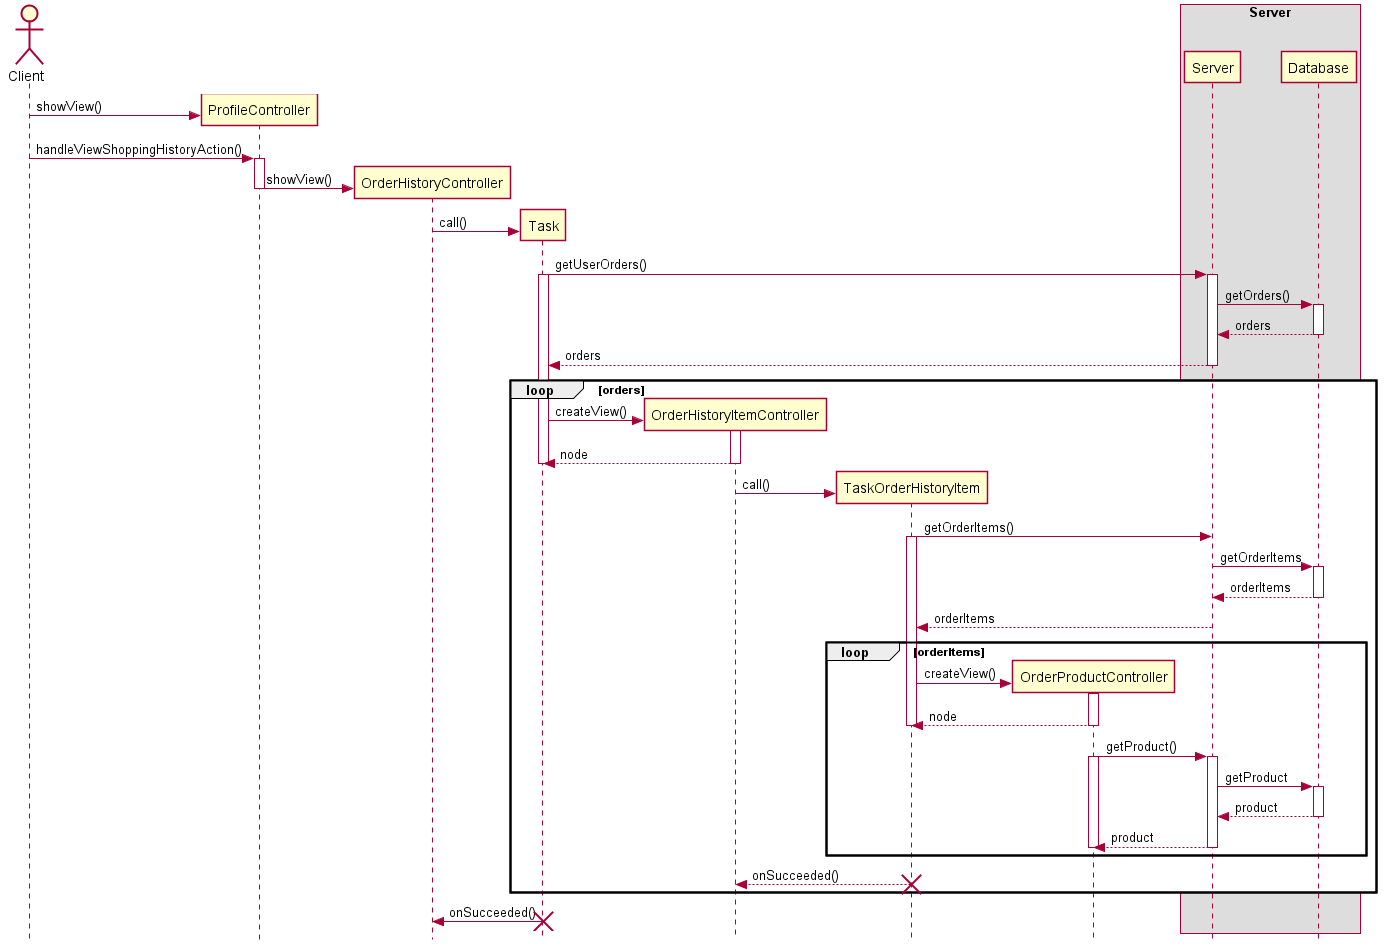
\includegraphics[width=0.9\textwidth]{shopping_history_sequence.png}
  \caption{Sequence diagram Storico Spese}
\end{figure}

\newpage

\section{Design Patterns}

\subsubsection{Singleton}	

Il pattern Singleton viene utilizzato per garantire uno stato globale alle
istanze del Database e della Sessione dell'utente. L'utilizzo di questo pattern
è necessario in queste due classi ma si è cercato di evitarne l'utilizzo in
altri contesti per evitare che la staticità della classe rendesse impossibile
il mocking durante il test. In particolare, nella \textbf{Sessione} viene
tenuta un istanza della classe Utente per gestire tutti i dati relativi
all'utente autenticato; nel \textbf{Database} tutti i modelli utilizzano la
stessa istanza per creare una connessione al database SQLite. 

\subsubsection{Factory Utente}

Abbiamo creato una classe astratta Utente con un metodo \verb|redirect()|
astratto, le classi Client e Manager estendono Utente e ne implementano il
metodo. Mentre la classe FactoryUtente permette di generare un'istanza delle
due classi in base alle credenziali fornite. Quindi quando il metodo
\verb|redirect()| verrà chiamato si verrà indirizzati rispettivamente alla
pagina del Cliente o del Manager.

\subsubsection{DAO Observable Sessione}

Molte views e task devono poter accedere ai dati del carrello e della sessione
utente durante la fase di acquisto. Più di un thread accede nello stesso
momento agli stessi dati, per questo è necessario utilizzare una DAO (Data
Accesses Object) per evitare possibili TOCTOU (Time Of Check Time Of Use) e
race condition (osservate durante lo sviluppo).

\subsubsection{Prodotto}

AbstractProduct, Prodotto and ROProduct (Read Only Prodotto)


% Tasks & Components
\chapter{Discussione}

\section{Test suite}

Tutti i test sono stati fatti in JUnit, a parte quelli per le funzioni di
JavaFX che sono stati eseguiti manualmente.

% TDD crea test, crea funzione intellij genera metodi
% Unit test tutto server, code coverage
% Javafx non testabile, ma funzioni attorno si
% CI/CD GitHub test automatici

\section{Conclusione}

Il progetto è stato condotto cercando inizialmente di rispettare le metodologia
\textbf{Scrum} e utilizzando un \textbf{System Version Control} quale GIT per
poter gestire al meglio il lavoro a distanza sullo stesso progetto. Dopo aver
concordato degli sprint molto ristretti (una settimana circa) e avendo un brief
ogni due giorni invece che 1, abbiamo cominciato col progetto.

\end{document}
